\chapter{Hand Motion Models}
\label{C:hand-model}

This chapter puts together the learnings from the previous chapters to develop neural network-based models for hand motion modeling.

\section{Introduction}

Hand motion modeling is a task which involves predicting hand poses (ie. configurations of joints, as described in \Cref{s:hand-config}), across many timesteps in an animation. This is a challenging task because of the large number of degrees of freedom in the hand, the large number of timesteps in an animation, and the fact that the hand is a complex structure where small errors are easily noticable.

This chapter presents two models which are able to predict hand poses. They are both trained on a dataset of 3D hand animations produced via motion capture, and are able to predict hand poses in a variety of different poses. The first model is trained with a regression objective, and is able to predict whole hand poses. The second model is trained with a parameter estimation objective, and is able to predict the parameters of a von-Mises distribution over individual joints in the hand. This model is then auto-regressively called to predict the whole hand pose.

\section{Previous Work}
\label{s:prev-work}

To my knowledge this work is the first to target this exact task, but there are two closely related areas of previous work which are relevant to this chapter. The first is the use of neural networks for pose estimation, and the second is the use of neural networks for human motion modeling.

\subsection{Pose Estimation}
\label{ss:pose-estimation}

Pose estimation (eg. \cite{real-time-hand-modeling}) is the task of estimating the pose/configuration of a character or hand from image or video data. Almost all the work in the literature related to hand motion is some variant of hand pose estimation task -- this is because it is directly applicable to virtual reality (VR) applications.  The task of hand motion modeling is often downstream of hand pose estimation -- the output of a hand pose estimation model is often used as input to a hand motion model. This is the case for the ManipNet dataset \cite{manipnet}, which is used in this thesis.

An example of hand pose estimation is shown in \Cref{fig:pose-estimation}. The input to the model is a single image of a hand, and the output is a 3D pose of the hand. The model is able to predict the pose of the hand in a variety of different poses, including poses which are not in the training data.

\begin{figure}
    \begin{minipage}{0.48\linewidth}
        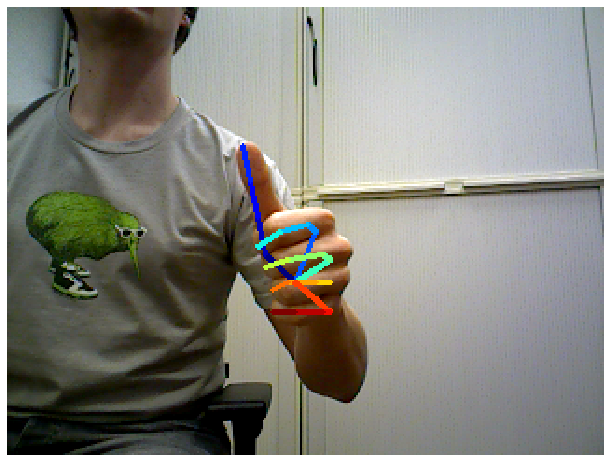
\includegraphics[width=\linewidth]{figures/hand-pose-1.png}
    \end{minipage}
    \hfill
    \begin{minipage}{0.48\linewidth}
        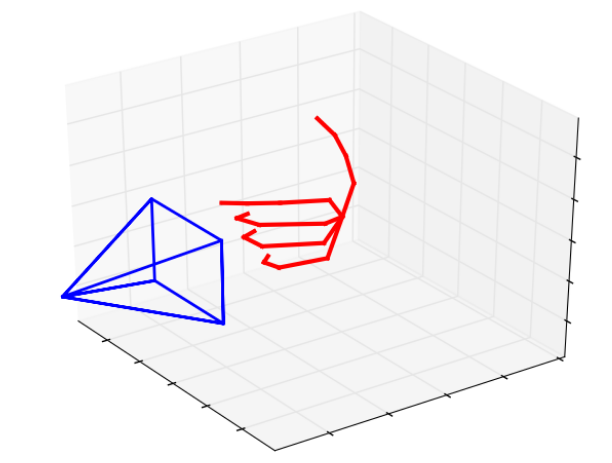
\includegraphics[width=\linewidth]{figures/hand-pose-2.png}
    \end{minipage}
    \captionsetup{parskip=7pt}
    \caption[Hand pose estimation]{An example of the hand pose estimation task, from \cite{zimmermann2017learning}. Left: The input to the model is an image or video of a hand. Right: The output is a 3D pose of a hand.}
    \hrulefill
    \label{fig:pose-estimation}
\end{figure}

\subsection{Human Motion Modeling}
\label{ss:human-motion-modeling}

Human motion modeling is the task of predicting human motion from past motion data. We can divide this into three rough categories, as per \cite{human-motion-modeling-survey}:
\begin{enumerate}
    \item Human motion prediction, which is the task of predicting future human motion given an observed sequence of human poses.
    \item Human motion control, which is the task of producing a sequence of realistic human motion given some goal, eg. a target pose, or a target trajectory.
    \item Cross-modal motion synthesis, which is the task of producing a sequence of human motion given some other input, eg. a sequence of images, or a sequence of audio. This overlaps with pose estimation, because the input to the model is often video data.
\end{enumerate}

\begin{figure}
    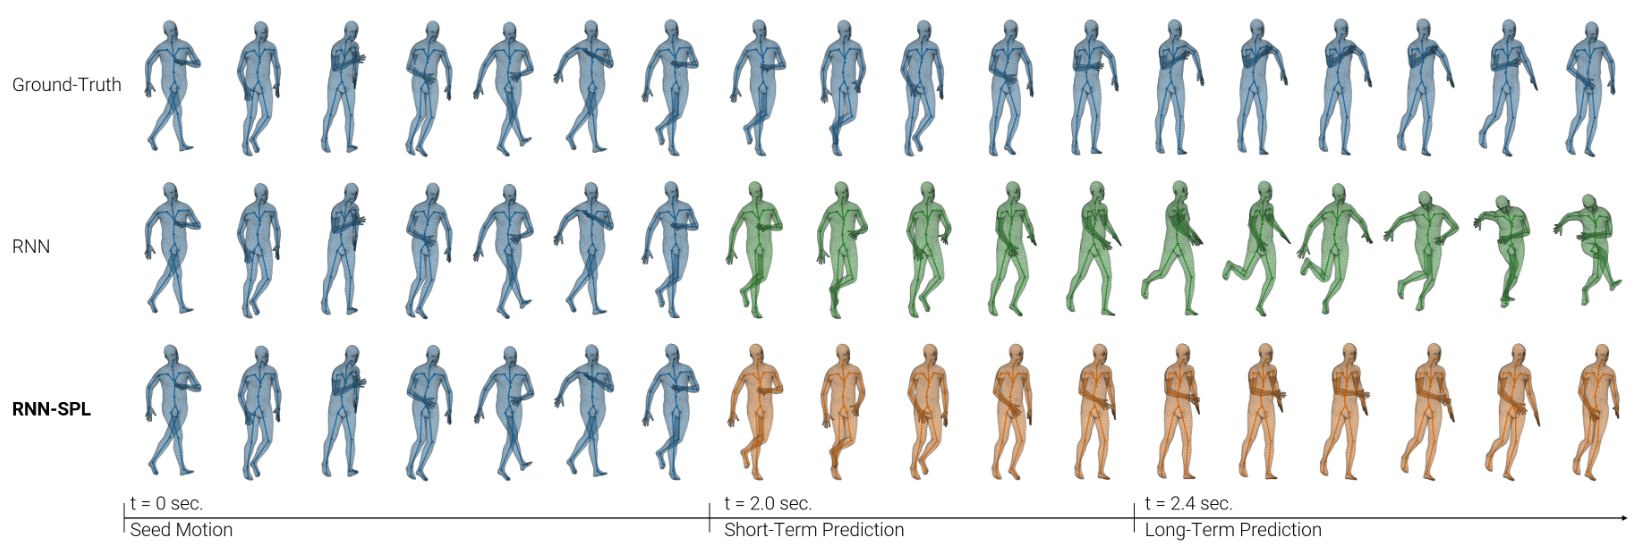
\includegraphics[width=\linewidth]{figures/character-motion-modeling.png}
    \captionsetup{parskip=7pt}
    \caption[Character motion modeling]{An example of the character motion modeling task, from \cite{structured-prediction}. Top: Ground truth motion sequence, typically recorded via motion capture. Middle and bottom: Two different completions of the motion sequence, produced by a model.}
    \hrulefill
    \label{fig:character-motion-modeling}
\end{figure}

Most of the literature in this area is focused on character motion, ie. predicting the pose of the body and limbs, rather than the hands or facial expression, although there is also a reasonable body of work on lipsyncing. For example, there are a number of recent papers on modeling choreographed dancing, which treats character motion as a sequence-to-sequence task, generating a sequence of poses conditional on a music track \cite{dance-choreonet}. Recent works here use encoder-decoder transformers for this purpose, for example \cite{dance-transflower}. 

Of the many related works, the most relevant ones are the following:
\begin{itemize}
    \item ManipNet \cite{manipnet}, whose high-fidelity motion capture dataset is used in this chapter, although their task is very different. Their work is unique and focuses on predicting the pose of the fingers based on the pose of only the wrist and the pose and geometry of a held object.
    \item \cite{structured-prediction}, who focus on predicting character motion. The task in this chapter is identical to their character motion modeling task shown in \Cref{fig:character-motion-modeling}, except that of course they work with character poses rather than hand poses.
    \item SignBERT \cite{signbert}, which focuses on training a ``language model'' for sign language, using hand pose sequences extracted from video datasets of sign language using hand pose estimation. The work in this chapter is very similar to this, except that SignBERT uses an encoder-only transformer and a masked sequence modeling pretraining task, whereas the work in this chapter uses a decoder-only model and an autoregressive sequence modeling pretraining task. Additionally, the dataset used in this chapter is captured with a high-fidelity motion capture system, rather than derived from video data.
\end{itemize}

\section{Dataset}
\label{s:dataset}

The dataset used for the experiments in this chapter is the ManipNet \cite{manipnet} dataset. This dataset was captured using a \textit{deep label} system \cite{deep-labeling}, and an \textit{Optitrack} \cite{optitrack} motion capture system with 16 cameras at 60 frames per second, and gloves with 19
markers per hand for finger tracking.

The dataset contains 62 animation sequences, each of which involves a participant (whose hand and joint position is being recorded via a motion capture setup) manipulating a rigid object such as a block, teapot or mug. Each animation sequence contains somewhere between 4000 frames (2m 20s at 30 frames/s) and 8000 frames (4m 40s) of data.

The data was split into a training set, validation set, and test set. The lengths of these splits along with some other statistics about the dataset can be seen in \Cref{tab:manipnet-stats}. The test set was used for producing visualizations and for the final evaluation of the models, and the validation set was used to tune hyperparameters and for determining early stopping point when training.

The data is represented in the BVH (BioVision Hierarchy) format \cite{bvh}. A BVH file is a text file which contains the definition of a hierarchy of joints, including the offset and rest pose, followed by data for each frame of the animation. Each ManipNet BVH file contains 51 floating point values per frame (14 joints $\times$ 3 values per joint). The two hands are specified in two different files.

\begin{table}
\centering
% table of loss values
\begin{tblr}{ l r r r r }
    \hline
    & Total & Train & Val & Test \\
    \hline
    N° frames & 467372 & 375372 & 44000 & 48000 \\
    N° examples & 62 & 50 & 6 & 6 \\
    Length & 4h 19m & 3h 28m & 24m & 26m \\
    Mean $\amse$ & & 0.0737 & 0.0555 & 0.0818 \\
    \hline
\end{tblr}
\caption[Statistics of ManipNet dataset]{Summary statistics for the ManipNet \cite{manipnet} dataset used in the experiments. The $\amse$ statistic shows the error on the respective dataset if a model simply predicts the \textit{circular mean} (\Cref{eqn:circ-mean}) of all the frames in the training set. This represents an upper bound (and sanity check) on the error for the experiments.}
\hrulefill
\label{tab:manipnet-stats}
\end{table}

\section{Training the deterministic models}
\label{S:mean-model}

The first models are deterministic models that were trained with a regression loss, to predict a whole hand pose at each timestep.

\subsection{Tasks}

Two models were trained with identical hyperparameters on two tasks. Both models were trained to minimize the angular mean squared error $\amse$ (\Cref{eqn:amse}) between the predicted pose and the ground truth pose. As a result of using this training objective, the outputs of the models estimate the expectation over the posterior distribution of the hand pose at the next frame, given the previous frames.


The first task was a plain auto-regressive pre-training task as in \Cref{ss:autoreg-pretraining}. Specifically, the task was to predict the pose of the hand at the next frame, given some number of previous frames.

The second task was as above but with the addition of a goal condition. Specifically, the task was to predict the pose of the hand at the next frame, given some number of previous frames and a goal pose. The goal pose was the pose of the hand at the last frame of the sequence, and was prepended to the input sequence of every training example.

The data was provided to the model as a sequence of 204-dimensional vectors (2 hands $\times$ 17 joints $\times$ 3 unit vectors per joint $\times$ 2 components per unit vector), and the model was trained to predict the outputs of the subsequent timestep (another 204-dimensional vector).


\begin{table}
\centering
\begin{tblr}
    {
        vlines,
        rows={m},
    }
    \hline
    N° input dims & 204 \\
    N° output dims & 204 \\
    N° embedding dims & 256 \\
    N° layers & 24 \\
    N° hidden dims & 512 \\
    N° attention heads & 8 \\
    Total N° parameters & 56,977,304 \\
    Batch size & 16 \\
    Chunk length & 512 \\
    GPU & NVIDIA RTX 3080 \\
    Training steps & 20,000 \\
    { \bf Task 1} \\
    Training time & \approx 19m \\
    Training $\amse$ & 0.000456 \\
    Validation $\amse$ & 0.0448 \\
    {\bf Task 2} \\
    Training time & \approx 19m \\
    Training $\amse$ & 0.000447 \\
    Validation $\amse$ & 0.0480 \\
    \hline
\end{tblr}
\caption[Training details for the deterministic hand motion models]{Hyperparameters and training configuration for the deterministic models.}
\label{tab:mean-model-hyperparams}
\end{table}

The details of the training and hyperparameters are shown in \Cref{tab:mean-model-hyperparams}.

\subsection{Results}
\label{ss:mean-model-results}

The results are presented in two formats: image visualizations in \Cref{fig:mean-images}, and a video visualization on YouTube (see \Cref{fig:mean-video}). Both visualizations show the model's predictions at each timestep, and the ground truth at each timestep.

\begin{figure}
    \centering
    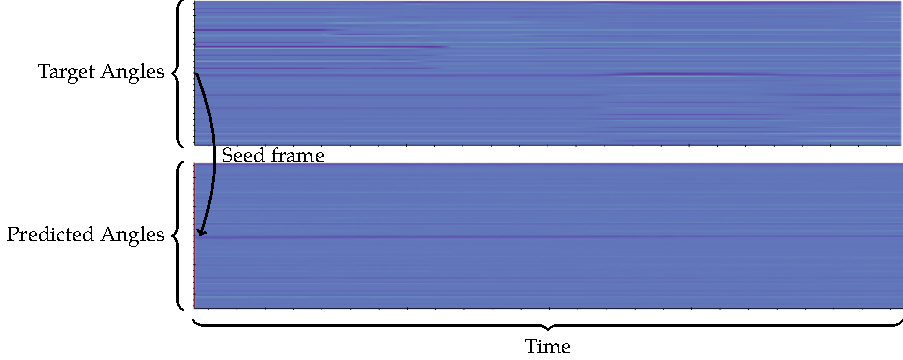
\includegraphics[width=\linewidth]{figures/mean-untargeted.pdf}

    \vspace{1cm}

    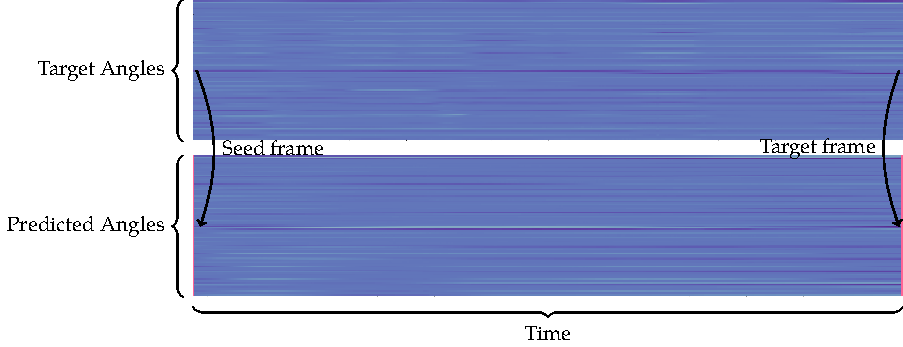
\includegraphics[width=\linewidth]{figures/mean-model-1-predictions.pdf}
    \captionsetup{parskip=7pt}
    \caption[Deterministic model predictions]{Image visualizations of outputs from the deterministic model. Top: Predictions from the untargeted model. Bottom: Predictions from the model trained on the target pose problem.

    The above 102px by 512px images show two pairs of predicted animation sequences. The top image of each pair shows the ground truth data, and the bottom image shows the model's predictions.

    The predictions were produced by seeding the model with either the first frame of the ground truth data then auto-regressively predicting the hand poses at each timestep in between. In the bottom figure, the model is also provided the final frame of data as a target. We can see that in both cases the model initially correctly predicts poses close to the ground truth, but it then diverges.}
    \label{fig:mean-images}
\end{figure}

\begin{figure}
    \centering
    \href{https://www.youtube.com/watch?v=XxVlzT4joAU}{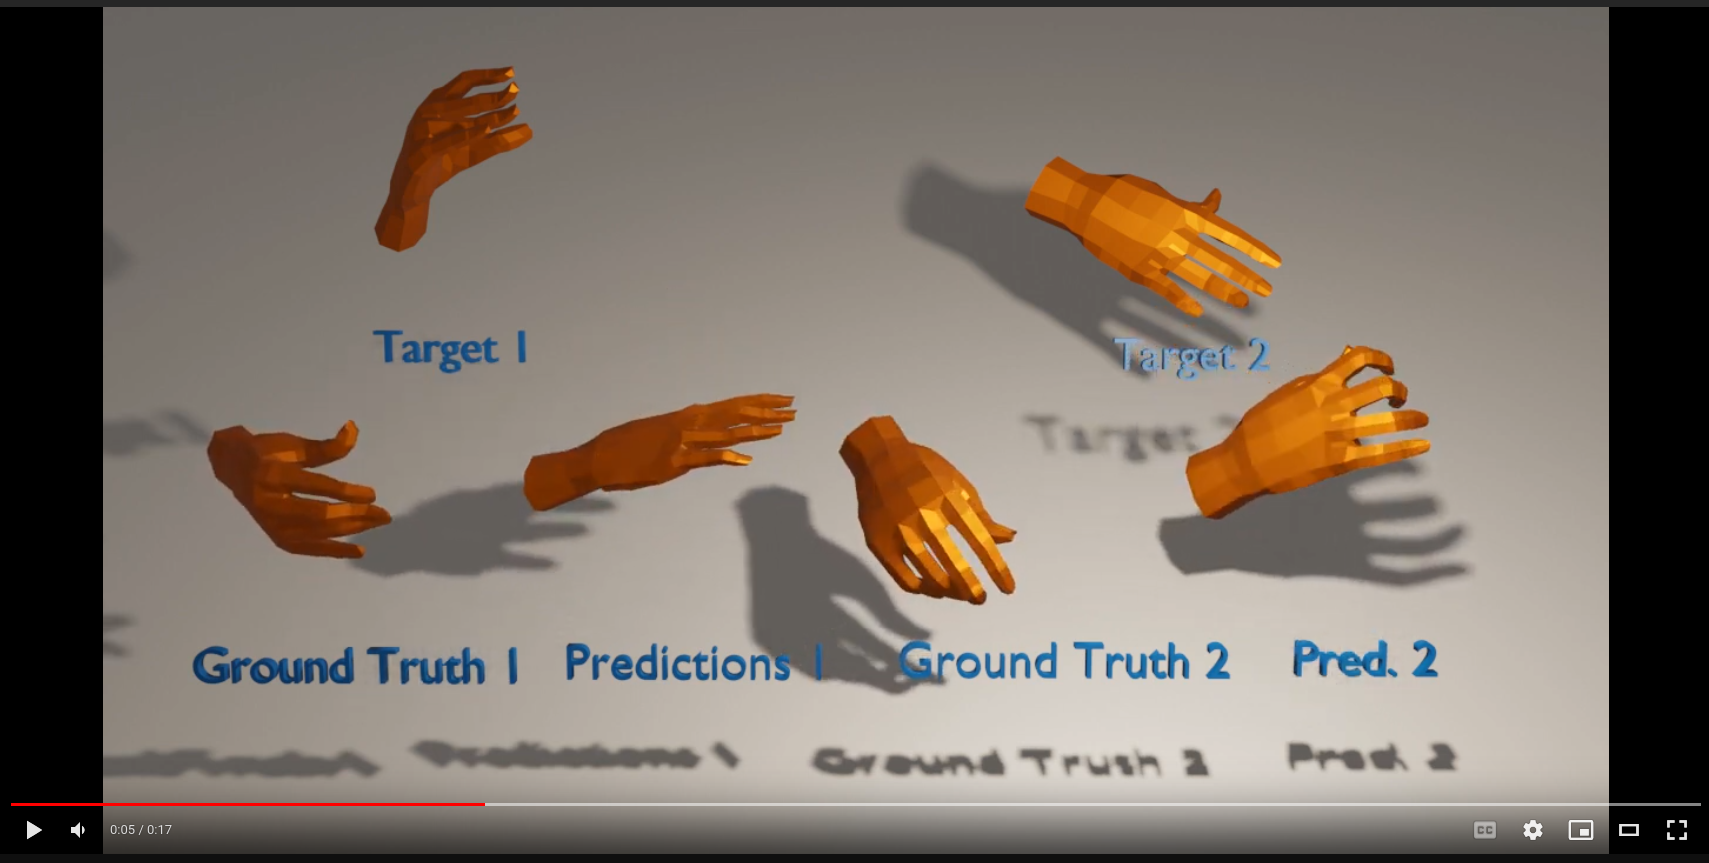
\includegraphics[width=\linewidth]{figures/youtube-thumbnail.png}}
    \captionsetup{parskip=7pt}
    \caption[Video of the deterministic model predictions]{Video visualizations of outputs from the deterministic model (On the targeted task only). A video showing the results as rendered animated hands can be found \href{https://www.youtube.com/watch?v=XxVlzT4joAU}{here}. The video shows two different ground truth seed sequences, and the model's predictions for each.}
    \label{fig:mean-video}
\end{figure}

\clearpage

As we can see in the figures and video, both models produce relatively smooth and realistic predictions. However, the model trained on the targeted task does not achieve the objective. Despite the target pose being provided during both training and the prediction process, the predictions do not re-converge to the target pose at the end of the predicted sequence. This may be because the model has not learned to use the target pose, which might happen if the model has over-fitted to the training data. Over-fitting is also suggested by the difference between the training and validation $\amse$ values (\Cref{tab:mean-model-hyperparams}). The training loss is significantly lower than the validation loss.

\section{Training a probabilistic model}
\label{S:prob-model}

The second model was trained with a parameter estimation objective, to predict the parameters of a von-Mises distribution over individual joints in the hand.

\subsection{Task}

Unlike the previous model where the data was provided as sequences of whole frames, for the probabilistic model the data was provided as a sequence of single 2D unit vectors. This is neccessary in order to model the joint probability distribution of a hand pose. Each unit vector represents a single component angle of a single joint in the hand. The model was then trained to predict the parameters of a von-Mises distribution over the next component angle, using the von-Mises negative-log-likelihood as the loss function. The model is called 51 times to produce all of the component angles for one frame of the animation, then this is repeated for each frame in the sequence.

Because the data was provided as a sequence of single components rather than full pose vectors, the probabilistic model requires a much longer sequence length to condition the model on the same amount of data from the animation. Because the transformer attention matrices scale in memory complexity with the sequence length, training the probabilistic model was limited by the available GPU memory. In order to keep a long context window and still fit into the GPU memory during training, the model is therefore smaller than the deterministic model.

\subsection{Results}
\label{ss:prob-model-results}

As before, the results are presented as both image visualization in \Cref{fig:prob-images}, and video visualization in \Cref{fig:prob-video}. Both show a comparison between the model predictions and the ground truth data.

\begin{table}
    \centering
    \begin{tblr}
        {
            vlines,
            rows={m},
        }
        \hline
        N° input dims & 2 \\
        N° output dims & 2 \\
        N° embedding dims & 510 \\
        N° layers & 3 \\
        N° hidden dims & 1048 \\
        N° attention heads & 8 \\
        Total N° parameters & 23,710,750 \\
        Batch size & 16 \\
        Chunk length & {1530 \\ (30 frames $\times$ 51 components)} \\
        Training time & 12m 9s \\
        Training steps & 10,000 \\
        \hline
    \end{tblr}
    \caption[Training details for the probabilistic hand motion model]{Hyperparameters and training configuration for the probabilistic model.}
    \label{tab:prob-model-hyperparams}
\end{table}

\begin{figure}
    \centering
    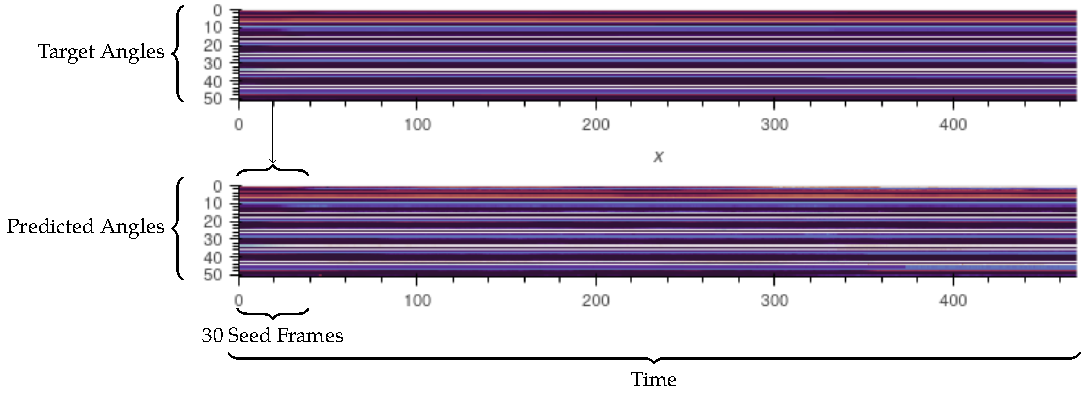
\includegraphics[width=\linewidth]{figures/probabilistic-model-predictions.pdf}
    \captionsetup{parskip=7pt}
    \caption[Image visualizations of the probabilistic model]{Image visualizations of outputs from the probabilistic model. The above 51px by 450px images show two animation sequences. The top image shows ground truth data, and the bottom image shows the model's predictions. The first 30 frames of the predicted sequence are copied from the ground truth as seed data, and the remaining frames are predicted by the model.}
    \label{fig:prob-images}
\end{figure}

\begin{figure}
    \centering
    \href{https://www.youtube.com/watch?v=moExsVteA-A}{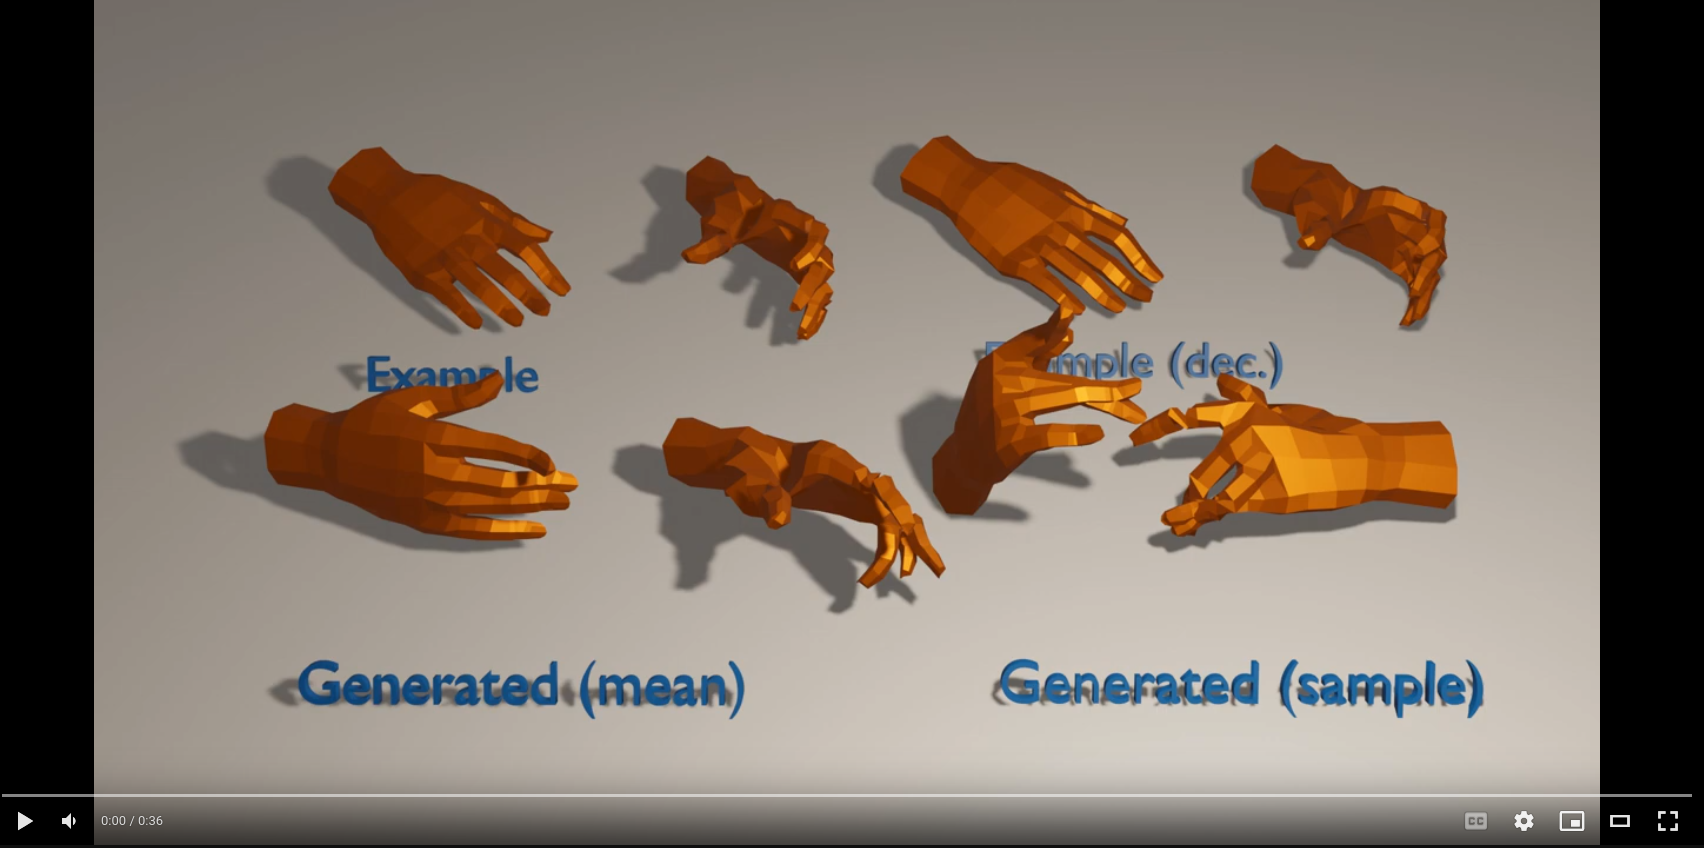
\includegraphics[width=\linewidth]{figures/probabilistic-model-video-thumbnail.png}}
    \captionsetup{parskip=7pt}
    \caption[Video visualizations of the probabilistic model]{
        Video visualizations of outputs from the probabilistic model. A video showing the results as rendered animated hands can be found \href{https://www.youtube.com/watch?v=moExsVteA-A}{here}. The video shows two different ground truth seed sequences, and the model's predictions for each.}
    \hrulefill
    \label{fig:prob-video}
\end{figure}



We can see from the figures and video that the probabilistic model unfortunately does not perform well. There are two main problems:
\begin{enumerate}
    \item The sampling process is unstable, and the fingers rapidly converge into an unusual part of the hand pose space.
    \item The model predicts distributions with high variance, resulting in flickering / noise when sampling. This is especially noticeable in the wrist, where it causes the whole hand to shift.
\end{enumerate}

\section{Discussion}

The deterministic model performs better than the probabilistic model -- it is able to produce smooth animations, while the probabilistic model produces flickering/noise and also degrades as the sampling process progresses.

The difference in performance may be due to the difference in difficulty on the respective problems. Because the probabilistic model predicts individual component angles, it effectively has a 100$\times$ longer sequence length. In addition it is trained with a parameter estimation objective, rather than a reconstruction objective, which may be more difficult to optimize - in particular the $\kappa$ (concentration) paramter of the von-Mises distribution.

To determine whether the difference in performance is due to the model architecture, or the training objective, a third model could be trained with the $\amse$ loss, but on the sequence-of-single-components task. However, due to time constraints this was not done.

Additionally, it was only recently that the smooth results of the deterministic model were achieved, and due to time constraints the probabilistic model was not retrained to match the deterministic model's hyperparameters. As a result, it is possible that the probabilistic model could be yet improved to be competitive by retraining it with similar hyperparameters to the deterministic model.


\section{Conclusions and Future Work}

This chapter has presented two classes of transformer models on hand motion modeling tasks.

The first models are trained with a regression objective, and are able to produce smooth animations, but are not able to be conditioned on a target pose, possibly due to overfitting. Future work would be to investigate training smaller models and regularization techniques to prevent overfitting (and so determine whether this is the issue). If so, then additional datasets (such as the sign language dataset from \cite{signbert}) could be used to increase the model's generalization ability.

The second model is trained to predict the parameters of a von-Mises distribution over individual component angles of a hand pose. Unfortunately, the model performs poorly and the conclusion is inconclusive. Future work here would include:
\begin{enumerate}
    \item Further hyperparameter tuning.
    \item Training a deterministic model on the sequence-of-single-components task, to determine whether the difference in performance is due to the different task, or the different training objective.
\end{enumerate}
